% ****** Start of file apssamp.tex ******
%
%   This file is part of the APS files in the REVTeX 4.2 distribution.
%   Version 4.2a of REVTeX, December 2014
%
%   Copyright (c) 2014 The American Physical Society.
%
%   See the REVTeX 4 README file for restrictions and more information.
%
% TeX'ing this file requires that you have AMS-LaTeX 2.0 installed
% as well as the rest of the prerequisites for REVTeX 4.2
%
% See the REVTeX 4 README file
% It also requires running BibTeX. The commands are as follows:
%
%  1)  latex apssamp.tex
%  2)  bibtex apssamp
%  3)  latex apssamp.tex
%  4)  latex apssamp.tex
%
\documentclass[%
reprint,
%superscriptaddress,
%groupedaddress,
%unsortedaddress,
%runinaddress,
%frontmatterverbose, 
%preprint,
%preprintnumbers,
%nofootinbib,
%nobibnotes,
%bibnotes,
 amsmath,amssymb,
 aps,
%pra,
%prb,
%rmp,
%prstab,
%prstper,
%floatfix,
]{revtex4-2}

\usepackage{subfiles}
\usepackage{graphicx}% Include figure files
\usepackage{dcolumn}% Align table columns on decimal point
\usepackage{bm}% bold math
\usepackage{float}
\usepackage{mathtools}
\usepackage{xcolor}
\usepackage{physics}
\usepackage{tcolorbox}
\usepackage{tensor}
\usepackage{hyperref}% add hypertext capabilities
%\usepackage[mathlines]{lineno}% Enable numbering of text and display math
%\linenumbers\relax % Commence numbering lines

%\usepackage[showframe,%Uncomment any one of the following lines to test 
%%scale=0.7, marginratio={1:1, 2:3}, ignoreall,% default settings
%%text={7in,10in},centering,
%%margin=1.5in,
%%total={6.5in,8.75in}, top=1.2in, left=0.9in, includefoot,
%%height=10in,a5paper,hmargin={3cm,0.8in},
%]{geometry}

\newcommand{\Hp}{\mathcal{H}}
\renewcommand{\thesection}{\arabic{section}}
\renewcommand{\thesubsection}{\thesection.\arabic{subsection}}
\renewcommand{\thesubsubsection}{\thesubsection.\arabic{subsubsection}}
\makeatletter
\def\@date{\Dated@name\@date@value}
\def\Dated@name{Date: }
\makeatother
\renewcommand{\figurename}{Fig.}
\renewcommand{\tablename}{Table}
\makeatletter
\renewcommand{\subsubsection}{%
	\@startsection
	{subsubsection}%
	{3}%
	{\z@}%
	{.8cm \@plus1ex \@minus .2ex}%
	{.5cm}%
	{\normalfont\small\centering}%
}
\makeatother

\begin{document}

\title{The Large Scale Structure of the Cosmic Microwave Background}

\author{E. B. Rørnes}
 \email{e.b.rornes@fys.uio.no}
\affiliation{Institute of Physics, University of Oslo,\\0371 Oslo,  Norway}

\date{\today}

\begin{abstract}
In this paper we present everything needed to create a Boltzmann-Einstein solver which calculates the Cosmic Microwave Background (CMB) power spectrum in a simplified Lambda-Cold-Dark-Matter model. This is done by considering linear perturbations to the Friedmann-Lema\^itre-Robertson-Walker cosmology in the Newtonian gauge. First the completely flat background cosmology is computed where we later analyze recombination epoch. Finally we linearly perturb the background and compute the CMB and matter power spectrum. The formation of heavier atoms than hydrogen together with the effects of polarization and neutrinos are ignored throughout. This yields a rather significant discrepancy for small scale modes compared to more sophisticated methods, but is however accurate enough to understand the underlying mechanisms behind the CMB. The main results include: 1) various important epochs which are numerically calculated from the fiducial background cosmology, 2) the recombination history of the Universe, 3) how perturbations from initial conditions stemming from inflation allowed for overdensities to form large scale structures, and 4) a theoretical prediction to the CMB and matter power-spectra.
\end{abstract}

\keywords{cosmic microwave background  --	large-scale structure of Universe}
\maketitle

\tableofcontents
\newpage
\section*{Introduction}
The cosmic microwave background (CMB) radiation is the oldest source of information that we currently have access to in our universe. This is then a vital piece of measurement which we can use to probe the evolution of the entire universe at very large scales. Today we observe that the temperature of the CMB photons coming from every direction is nearly the same with only minor fluctuations of order $\sim10^{-5}\,$K. These photons, in a classical model, would have no possibility of causally interacting with one another to reach such an equilibrium. So the question is then; how did the photons coming from all directions in the sky become the same temperature? And why are there even any fluctuations at all? These are the main questions this paper will attempt to answer.

The overarching goal is to create a Boltzmann-Einstein solver which can numerically predict the CMB power spectrum and CMB map that we observe through observations. Along the way we will find many interesting results which require us to include both dark matter and dark energy as the current understanding of the evolution of the universe is not possible without these given current models. To do this we will first be starting off with the completely isotropic and homogeneous background cosmology in a so-called Lambda-Cold-Dark-Matter universe in section \ref{sec:1}. In section \ref{sec:2} we will move over to probing the era of recombination. This is the time where neutral atoms begin to form as the energy density of the universe decays below a critical amount. Since the universe is neutral at this time, the photons decouple from the primordial plasma and are the CMB photons we see today. Next we will complicate our system by performing linear perturbations to the isotropic and homogeneous universe in section \ref{sec:3}. Here we will use various Boltzmann equations and Einstein field equations to get our hands on various differential equations whose initial conditions will be set via an inflation model. Finally in section \ref{sec:4} we will be in a position to actually achieve our main goal of this project; to compute the CMB spectrum.

This project was built on the template provided by \cite{AST5220LectureNotes} which already contains a large part of the structure behind the numerical parts of the project. We will simplify the entire process by neglecting neutrinos, reionization and any heavier elements than Hydrogen. As we will see this has a noticeable effect on the numerical data, but is still a relatively good approximation. We will however still compute the effects of neutrinos in the background cosmology in section \ref{sec:1}.

 In the entire paper the subscript 0 denotes today's values whilst a superscript 0 represents an equilibrium. Note that throughout the article there are many switches between natural units where $c=\hbar=k_b=1$ and SI units. 

% Include each milestone file

% Milestone I
\subfile{Milestone1/milestone1}

% Milestone II
\subfile{Milestone2/milestone2}

% Milestone III
\subfile{Milestone3/milestone3}

% Milestone IV
\subfile{Milestone4/milestone4}

\section{CMB map}
At last, with the values of $C_\ell$ from Fig. \ref{fig:C_ell} we can then create a CMB map given in Fig. \ref{fig:CMB_Map}. As mentioned in the implementations section this figure was generated by one of my co-students Anton Andreas Brekke who also created the corresponding colormap to match the various known CMB maps from actual data. 
\begin{figure*}[ht!]
	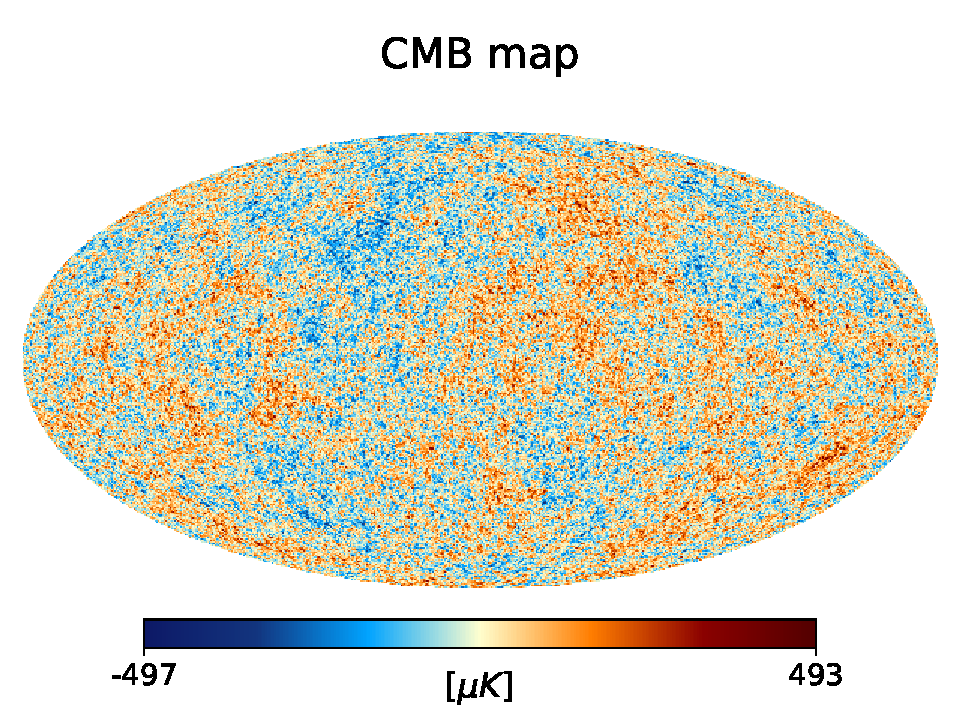
\includegraphics[width = \linewidth]{Milestone4/Figures/CMB_map.pdf}
	\caption{CMB map. Credits to Anton Andreas Brekke for creating the map and the corresponding cmap. Neither Healpy nor HealPIX would properly install for me, hence I was sadly not able to create this map myself.}
	\label{fig:CMB_Map}
\end{figure*}

\section{Conclusion}
In this project we solved the unperturbed FLRW background and determined various important epochs. We then took a deep dive into the recombination history of the universe where we determined the time when and at what scales one should expect to see the effects of the CMB photons. Further we perturbed the isotropic and homogeneous universe by using inflation as our model for initial conditions. At last we computed the famous CMB and matter power spectra. The data has a noticeable discrepancy from experimental data due to ignoring the effects of neutrinos, polarization, reionization and heavier elements than Hydrogen, but is overall still a worthwhile endeavor to be able to effectively comprehend the largest scales. Even without including the complications from the ignored effects we are still able to give a qualitative explanation of the underlying physics, explain the two main questions posed in the introduction and accomplish the main goal of creating a Boltzmann-Einstein solver for the CMB power spectrum.

\begin{acknowledgements}
	Many thanks to Hans Arnold Winther for providing detailed feedback on the various milestones together with his great website and programming template which make this project accessible for someone with a relatively poor programming background such as myself. Anton Andreas Brekke has also been a major help regarding talking through the various complicated subjects such that we both could get a better understanding of the underlying physics. This together with helping troubleshooting the various numerical programs needed for this project has been a major help.
\end{acknowledgements}

% Bibliography
\bibliographystyle{JHEP}
\bibliography{Master}

\end{document}
